\typeout{IJCAI-18 Instructions for Authors}

\documentclass{article}
\pdfpagewidth=8.5in
\pdfpageheight=11in
\usepackage{ijcai18}

\usepackage{times}
\usepackage{xcolor}
\usepackage{soul}
\usepackage[utf8]{inputenc}
\usepackage[small]{caption}
\usepackage{amsmath}
\usepackage{amsfonts}
\usepackage{parskip}
\usepackage{url}
\usepackage{amsthm}
\usepackage{tabularx}
\usepackage{graphicx}
\usepackage{hyperref}
\usepackage[inline]{enumitem}
\usepackage[title]{appendix}

\renewcommand\tabularxcolumn[1]{m{#1}}
\newcolumntype{Y}{>{\centering\arraybackslash}X}

\title{Confidence Based Poker Agents with Evolution Strategy Training - Group \#23}

\author{
Au Liang Jun, David Goh Zhi Wei, Law Yong Qiang Clinton, Lee Yiyuan, Tan E-Liang
\\ 
National University of Singapore
\\
\{e0203163, e0148854, e0175317, e0175089, e0177355\}@u.nus.edu
}
\begin{document}

\maketitle

\section{Introduction}
Poker is a non-deterministic, imperfect information game as neither the opponent's hole cards nor unrevealed community cards can be observed by a player. Given the pervasiveness of imperfect information in real world problems, from investment strategy to fraud detection \cite{brown2017libratus}, solving imperfect information games through Poker can give us insights as to what approaches could be adopted to better solve these problems.

We first identified key components of the game state which form the bases for our heuristics. Next, we developed heuristic-driven players with different decision making frameworks, including minimax trees, linear evaluations and neural nets. Through separate methods of genetic algorithms and stochastic optimisation using CMA-ES, we achieved faster convergence rates for the optimal weights for these heuristics and consequently better performances for our trained agents.

We also engineered a framework that allowed us to achieve tremendous speed ups in the training process. Overall, we were able to produce agents that perform consistently well (top 4) in the online tournaments against the other groups.

\section{Agent Design}
\subsection{Features}

Our designed players utilised features to make decisions heuristically. The following features (\(x_i)\) were considered and incorporated in the players' evaluation functions.

\begin{enumerate}
\item Hand strength: The expected win rate of the player's hole cards, combined with the community cards, if available. This is estimated via the Monte Carlo simulation.

\item Pot amount: As the goal of the agent is to earn the largest amount of money possible, the amount of money in the pot should influence its decision making. This value is normalised by dividing the current pot amount by the maximum possible pot which we determined to be \(64\times small\_blind\).

\item Payout: This feature models the likely payout of the game through \(hand\_strength \times pot\_amount\). \cite{Billings:1998:OMP:295240.295723}.

\item General Raises: Since we are unable to observe the opponent's hand, we incorporated the number of raises the opponent has made as a barometer of his hand strength.

\item Street: Advanced poker strategies exhibit slightly different behaviour for each of the different streets \cite{liley2010probability}. Since the implications of raising differ depending on what street they occur on,  instead of using a general weight for all raises, our agents use unique weights for raises on each street.

\item Aggression: It is possible for agents to develop a strong aversion to opponent raises, causing them to fold even if the opponent does not actually have a strong hand. Tracking how often opponents raises on average and injecting a bias to counter the aggression can help cautious agents perform better against aggressive opponents.
\end{enumerate}

\subsection{Linear Player}
In this approach, decisions are made based on a confidence level calculated via a linear combination of features. In particular, for a current game state with feature values \(X = (x_1, \dots, x_N)\), we have \[\operatorname{Confidence}(X) = \operatorname{Logistic}\left(\sum_{i = 1}^{N} w_i \cdot x_i \right)\] where \(w_i\) are weights assigned to each feature and \(\operatorname{Logistic}\) is a suitable activation function to scale the result to \((-1, 1)\). A decision is then made against threshold values, in particular \[\operatorname{Decision}(c) = \begin{cases} \operatorname{RAISE} & \text{if } c >\text{$rt$,}\\\operatorname{CALL} & \text{if }c > \text{$ct$ OR unable to Raise,} \\\operatorname{FOLD} &\text{otherwise,}\end{cases}\] where \(c\) = \(\operatorname{Confidence}(X)\), \(rt\) = Raise Threshold, \(ct\) = Call Threshold. Note that \(ct\) is not upper bounded by \(rt\) to allow for cases where \(rt < ct\).

\subsection{Minimax Player}
We concurrently explored the use of adversarial search for decision making.
In our implementation, the agent constructs a minimax tree at every call to \texttt{declare\_action()}. The general structure of the tree is illustrated in Figure \ref{minimaxtree}. 
\begin{figure}[h!]
\centering
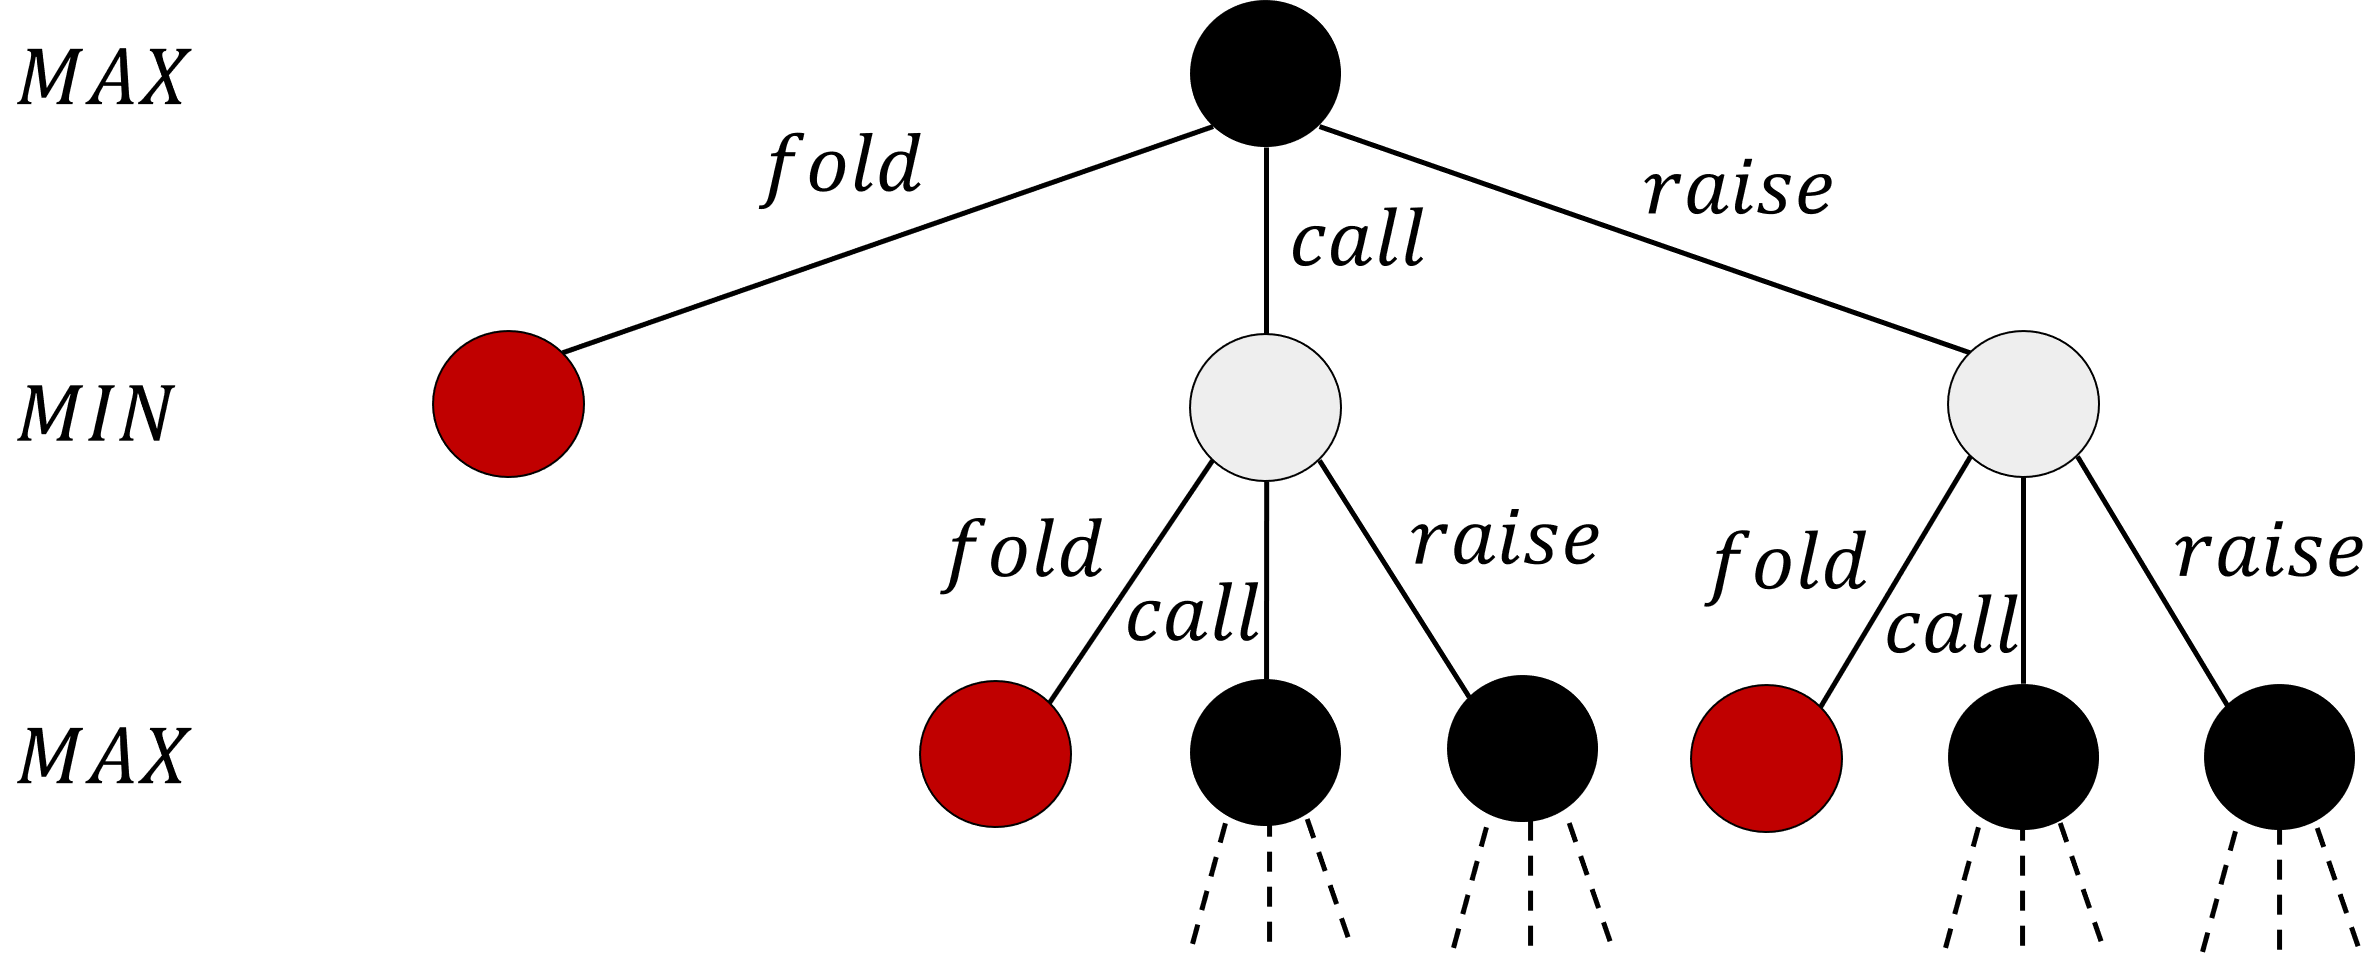
\includegraphics[width=8cm]{MinimaxTree}
\caption{Structure of Minimax Tree}
\label{minimaxtree}
\end{figure}

In the figure, the black nodes represent the max player, our agent, while the grey nodes represent the min player, our opponent. Each node in the tree holds information about the game state, used to generate child nodes and filtered to obtain features for evaluation. To reign in the branching factor, the different possible game states generated by the hidden cards are not incorporated in the form of chance layers. Instead, the opponent's hand and corresponding strength are only considered during the calculation of utility at terminal nodes.

Red nodes correspond to terminal nodes, which occur when either \begin{enumerate*}[label=(\roman*)] \item the action taken to reach it is a fold, \item the player has no further valid actions, or \item an imposed depth cut-off is reached\end{enumerate*}. At terminal nodes, utility is calculated as such:
\[\operatorname{Utility}(s) = \begin{cases}
\operatorname{Eval}(s) \cdot pot\_amount/2 &\text{if } \operatorname{In\_Edge}(s)
\\&\neq \operatorname{FOLD},
\\-pot\_amount/2 & \text{if } \operatorname{Parent}(s) \\&= \operatorname{MAX},
\\\phantom{-} pot\_amount /2 & \text{otherwise,} 
\end{cases}\]
where \(\operatorname{Eval()}\) is a modular function that can be modified to take on linear or neural functions, such as the Confidence() function of the Linear Player.

The edges in the tree represent actions taken by the player represented by the parent node. In our implementation, we utilise the \hyperlink{pypokerengine}{\emph{PyPokerEngine's}} \texttt{Emulator} class to simulate how a particular game state changes when a specific action is applied.

\section{Agent Training Methodology}
\subsection{Genetic Algorithm Based Training}
Since our final assessment would involve a single agent playing against a series of opponents in 1-versus-1 matches, we decided to model our training to maximise performance in this setting. We felt that a genetic algorithm best suited our training needs of swift convergence in a large, complex search space and good performance against a population of similarly competent agents \cite{DeJong1988}.

Our implementation involved generating a large number of \(n\) bots and arranging every bot to play a 1-versus-1 match against every other bot, resulting in a total of \(n \times (n-1)\) matches. The performance of a bot is determined by its overall win/loss ratio. Once all matches have been played, the weights with win/loss ratios \(>\) 1 are allowed to remain in training. All weights with win/loss ratios \(<\) 1 (i.e. more losses than wins) are removed and replaced with new weights. This technique allows us to optimise weights for multiple agents simultaneously.

\subsubsection{Agent weight generation}
Training a population of players with purely randomly generated weights raises a problem of efficiency as a majority of these weights result in weak players that are defeated by the most basic strategies. To accelerate convergence, we adopted a genetic method of weight generation. At the end of every training generation, the top performing weights are cloned and added into the training. Simultaneously, pairs of bots with high win rates are selected as parents to create a ``child" with the mean of their weights. We reason that this genetic approach of weight production will result in a faster convergence than generating completely random weights while continuing to explore the solution space.

To increase training efficiency and consistency, we seed the training with standardised players such as \hyperlink{raiseplayer}{\emph{RaisePlayer}}. This allows us to quickly cull weak weights as they would lose their matches against the seeded players. Also, it guarantees that the dominant players of the population will be able to beat standardised players. One potential disadvantage of this method is that we may be unable to escape a local minimum if the seeded players are too strong compared to the population. To mitigate this, we only introduce the seeded players after an arbitrary number of rounds to allow the randomly generated player population an opportunity to refine and evolve.

\subsubsection{Evaluation of trained agents}
The training cycle ends if the training exceeds an arbitrary number of generations in the interests of time. Once a cycle is over, we extract the best bots of the final generation and observe their performance against standardised players such as the \hyperlink{raiseplayer}{\emph{RaisePlayer}} and \hyperlink{randomplayer}{\emph{RandomPlayer}} as a measure of objective performance. As we trained stronger agents, we began to measure newly trained agents against the best of the previously trained agents as a benchmark test.

\subsubsection{Training evaluation}
The progress of this training method is observed through the average standard deviation across each weights in the agents with a positive win rate, referred to as \(\operatorname{WinStdDev}\). A low \(\operatorname{WinStdDev}\) indicates that the weights of winning agents are more homogeneous and is a sign of convergence. When \(\operatorname{WinStdDev}\) increases sharply after a period of consistent decrease, we read it as a sign of overfitting. We reason that if a population has begun to overfit, it will perform very well against other evolved agents, but lose badly against yet unseen randomly generated players. The only instance where \(\operatorname{WinStdDev}\) increases suddenly is when a weight set that is very different from the current dominant weights begins to win suddenly, \(\operatorname{WinStdDev}\), which causes the weights of winning players to be more varied. Thus, if \(\operatorname{WinStdDev}\) begins to diverge after a period of convergence, we interpret it as a sign of overfitting.

\subsection{CMA-ES Training}
In CMA-ES \cite{hansen2001completely}, a single hypothesis of the optimal player is tracked in terms of a multivariate normal distribution in the weight space. At each generation, samples are generated according to the current mean and variance, and based on the fitness of each sample, the mean and variance of the tracked hypothesis are modified according maximum likelihood updates.

An interesting property of CMA-ES is that it only requires the \textit{rank} of the samples rather than the absolute fitness values. In fact, the fitness values are discarded after determine the fitness ranking of the samples. As such, we only need to determine the relative performance among the sampled players in each generation.

Round robin matches are played among the samples, and the samples are ranked according to their win rate. In principle, we can build some suitable directed acyclic graph for the samples and determine a ranking via topological sort. However, this approach is unsuitable as cycles are typically produced due to the general lack of match transitivity.

\section{Agent Training Supporting Infrastructure}

We developed several tools and optimisation tweaks that allowed us to achieve extraordinary speed ups during training, as summarised in Table \ref{tab:speedups}.

\begin{table}[h!]
\small
    \centering
    \begin{tabularx}{\linewidth}{|Y|Y|} 
     \hline
     \textbf{Measure} & \textbf{Speed Up}\\
     \hline
     Parallelisation on SoC Compute Cluster & Ability to run up to \(2300\) games at once \\ 
     \hline 
     Perform Monte Carlo simulation for Win Rate Estimation in C/C++& Reduced time taken by a factor of \({\sim}180\).\\
     \hline
     Cython & Increases Python execution speed by about 22\% \\ 
     \hline
    \end{tabularx}
    \caption{Speed ups achieved from taken measures.}
    \label{tab:speedups}
\end{table}

\subsection{Parallelisation on SoC Compute Cluster}

As the games between separate pairs of players are entirely independent, we were able to parallelise our training games across the \hyperlink{computecluster}{\emph{SoC Compute Cluster}}. We engineered an architecture that could run multiple training algorithms and player designs simultaneously, thus allowing us to experiment widely and iterate quickly.

Games are supplied by a game server and processed by game clients spread across the 174 cluster nodes. The game clients are started with GNU Parallel \cite{Tange2011a} and communicate with the server over the network using the Eclipse Mosquitto \cite{ALight2017} implementation of MQTT, a lightweight and efficient machine-to-machine connectivity protocol. To ensure that we do not consume more resources than are known to be free and thus disrupt the tasks of other users, we scale our operations on each node based on their existing 5-minute load averages. Typically, our clients ran on anywhere between 1400-2300 CPU cores.

To illustrate the dramatic performance gains achieved, consider our internal evaluation tournament termed ``Botlympics", in which our best agents play a total of 9000 games against each other, for a total of \(9,000,000\) rounds of poker. On a single core, every 5000 rounds takes roughly 3 minutes to complete. A standard 4-core machine would require 22.5 hours to complete all the games, but 1400 CPU cores would take only about 20 minutes.

\subsection{Native Win Rate Estimation}

We re-implemented the win rate estimation calculations in C/C++ with the help of the OMPEval library \cite{timo:ompeval} for hand rank evaluations. The bridging between Python code and native code was done using Python's \texttt{ctypes} library. This approach greatly reduced the time taken for \(200\) Monte Carlo simulations from \({\sim}49.5\) ms to \({\sim}0.278\) ms on average, providing a \({\sim}180\)x speed up compared to the original implementation in \texttt{pypokerengine.utils.card\_utils}.

\subsection{Cython}

To further speed up the training process, we compiled our Python code using Cython \cite{behnel2010cython}. In 5 trials of a series of 5 games with a total of 4500 rounds of poker, the regular Python code averaged 23.86s per trial, while the Cythonised code averaged 18.55s per trial, a speed up of approximately 22.3\%.

\section{Results}
\subsection{Agent Performance}
\begin{figure}[h!]
\centering
\begin{tabular}{ |p{1.5cm}|p{1.5cm}|p{1.5cm}|p{1cm}|p{1cm}|  }
 \hline
 \multicolumn{5}{|c|}{\textbf{Top Bots}} \\
 \hline
 \textbf{Bot Name} & \textbf{Agent Class} & \textbf{Training Method} & \textbf{Games Won} & \textbf{Games Lost}\\
 \hline
WXMG3d & Linear & Genetic & 774 & 216\\
WXPr & Linear & Genetic & 752 & 238\\
CMA2TP2	& Linear & CMA-ES & 337 & 653\\
CMA2TP3	& Linear & CMA-ES & 328 & 662\\
Minmax3	& Minimax & Genetic & 158 & 832\\
Minmax4	& Minimax & Genetic & 153 & 837\\
 \hline
\end{tabular}
\caption{Win rates of selected bots in a round robin matchup. Each bot plays 30 games of 1000 rounds against 33 other bots.}
\label{winrate}
\end{figure}

Our experiments revealed that trained linear players performed the best, as it was the only agent design that was able to consistently defeat trained agents of different architectures as well as generic players such as RaisePlayer. Figure \ref{winrate} is an excerpt of the results of the internal tournament between all our trained agents.

\subsubsection{Minimax Player}
The trained Minimax Players did not perform as well as the linear agents. We attribute this to a number of factors:
\begin{enumerate}
   \item Restricted viable weight space: There was a need to scale the utility produced by evaluation functions to the deterministic utility of folding-induced terminal states. Failure to do so may result in a player with irrational behaviour, such as always choosing to fold. This greatly narrowed down the viable weight space available, and as such a Minimax Player typically needed to train for more generations to achieve comparable performance with a Linear Player with the same evaluation function. Furthermore, each match a Minimax Player takes relatively longer because the agent must perform graph creation and traversal for every decision.
   \item Poor time efficiency: Construction of the search tree was time-expensive even with $\alpha\beta$ pruning and action abstraction techniques. Despite the relatively small branching factor, a search cut-off had to be implemented in order to meet the specified agent reaction time. This limited the effectiveness of the minimax search.
   \item Invalid assumptions: The minimax search hinges on the assumption that the opponent is playing rationally and evaluating utility identically, a belief that allows the establishment of a Nash equilibrium. If the opponent is not acting rationally, or obtaining different utilities from game states compared to our agent, the minimax search would not produce a sequence of actions that models reality.
\end{enumerate}

% \subsubsection{Performance against other teams}
% We uploaded our agent (Group23Player) to the CS3243 tournament website on 2nd April 19. On the same day, it was able to win the tournament. Although our bot was subsequently beaten by other agents, it was consistently ranked among the top 4.
% On 17th April, we uploaded an updated version of our agent. In the 18th April tournament, our agent was the overall winner. It is worth noting that the final match was between two separate instances of our player, meaning that our agent bested both brackets of the tournament leading up to the finals.

\subsection{Training}
\subsubsection{Genetic algorithm method}
As mentioned in section 3.1, convergence is measured by the average standard deviation of each weight amongst winning bots or $WinStdDev$. Generally, the genetic training algorithm converged within 200 generations.

\begin{figure}[h!]
\centering
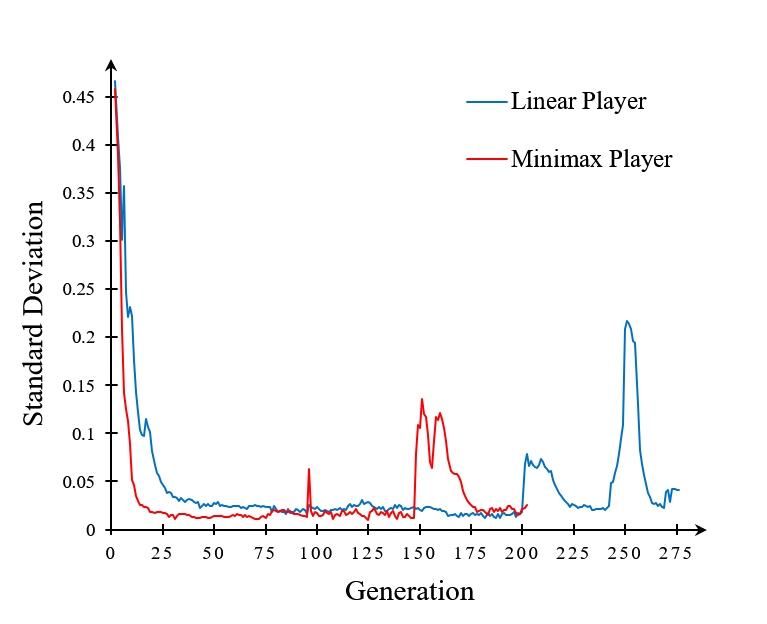
\includegraphics[width=7.5cm]{TrainingResultsConvergence2.png}
\caption{Convergence of Population-Based Training}
\label{convergence}
\end{figure}

A recurring problem was the risk of divergence when the previous generation of trained players were seeded into the training. While an increased $WinStdDev$ is to be expected with the introduction of strong players, this can result in overfitting as bots over-optimise to defeat the strong players and lose against weaker players. This trend can be observed in the Linear Player statistics in Figure 3. In this instance, the trained players were injected in generation 200. Although $WinStdDev$ recovers from the large spike at around generation 240, it never managed to converge to the value of \({\sim}0.025\) that was observed before generation 200.

\subsubsection{CMA-ES}
We keep track of the value of the step size during CMA-ES, which correlates directly to the variance of the tracked hypothesis for each weight. The algorithm converges at local minima before exploring other areas of the weight space multiple times (Figure \ref{cma}).

\begin{figure}[h!]
\centering
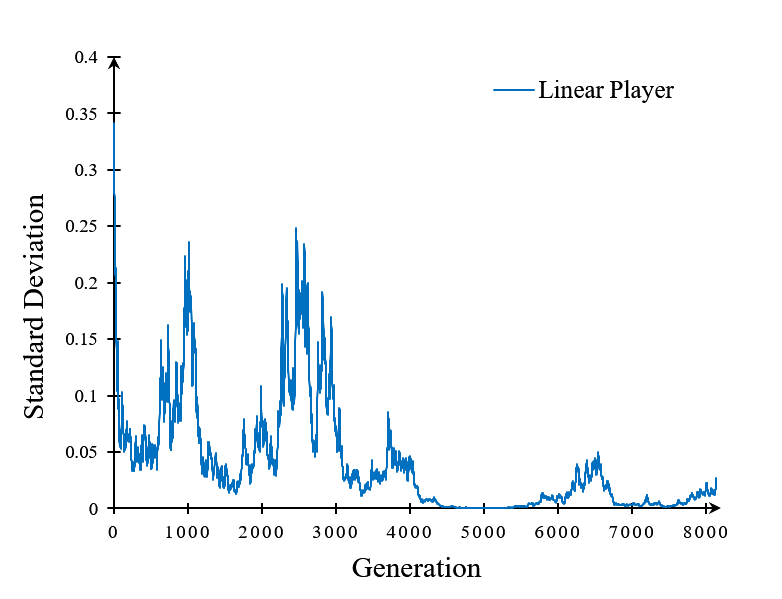
\includegraphics[width=7.5cm]{report/TrainingResultsConvergenceCMA.png}
\caption{Convergence of CMA-ES Training}
\label{cma}
\end{figure}

\section{Conclusion}
% We have shown that a trained linear player performed the best amongst various different players. Using a genetic algorithm to optimise weights proved to be the most efficient method. We managed to achieve excellent performance in the online tournaments with our trained player.

Our study finds that a trained linear player performs better than players with more sophisticated strategies, and our agent performed favourably in the online tournaments hosted by the CS3243 staff from March to April 2019, consistently ranking in the top 4. Furthermore, a genetic training algorithm is effective in performing reinforcement learning for the task, achieving convergence over a reasonable number of generations. We also attribute our agent's favourable performance to the efficient parallelisation of training, which enabled many variations of our agents to be trained across a large number of generations.

\newpage

\begin{appendices}

\section{Glossary}
\hypertarget{pypokerengine}{\textbf{PyPokerEngine}}: A Python library that we utilised as a framework for our poker playing AI. See \url{https://github.com/changhongyan123/mypoker}
\\\\\hypertarget{raiseplayer}{\textbf{RaisePlayer}}: A PyPokerEngine agent that always raises when it can. See \url{https://github.com/changhongyan123/mypoker/blob/master/raise_player.py}
\\\\\hypertarget{randomplayer}{\textbf{RandomPlayer}}: A PyPokerEngine agent that selects its action at random. See \url{https://github.com/changhongyan123/mypoker/blob/master/randomplayer.py}
\\\\\hypertarget{computecluster}{\textbf{SoC Compute Cluster}}: A collection of compute nodes provided by the NUS School of Computing. See \url{https://dochub.comp.nus.edu.sg/cf/services/compute-cluster}

\section{Neural Player}
We initially attempted to extend linear players by using neural networks to compute \(\operatorname{Confidence}(X)\) from feature values as a means of universal approximation to cover a larger class of possible mappings compared to just linear functions.

In the early stages of our project, the produced neural network based players generally performed better than linear players using the same base features. However, as more features were added, the number of weights in the neural network increased rapidly and the training became too infeasible for performant players to be produced.

\end{appendices}

\bibliographystyle{named}
\bibliography{ijcai18}
\end{document}

